\iffalse
\chapter{2016}
\author{AI24BTECH11022}
\section{me}
\fi

\usetikzlibrary{patterns}
\item A block of mass $m$ rests on an inclined plane and is attached by a string to the wall as shown in the figure. The coefficient of static friction between the plane and the block is 0.25. The string can withstand a maximum force of $20N$. The maximum value of the mass ($m$) for which the string will not break and the block will be in static equilibrium is \rule{1cm}{0.15mm} $kg$.

Take $\cos{\theta}=0.8$ and $\sin{\theta}=0.6$.

Acceleration due to gravity $g=10m/s^{2}$\hfill(2016)

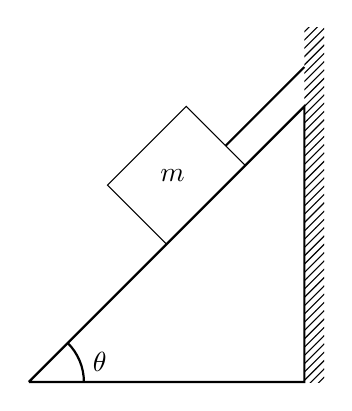
\begin{tikzpicture}
\draw[thick] (0,0) -- (3.5,0) --(3.5,3.5) -- (0,0);
\draw[thick] (2.5,3) -- (3.5,4);
\draw[thick] (0.7,0) arc[start angle=0, end angle=45, radius=0.7];
\node at (0.9,0.25) {$\theta$};
\fill[pattern=north east lines] (3.5,0) rectangle (3.75,4.5);
\draw (2.75,2.75) -- (2,3.5) -- (1,2.5) -- (1.75,1.75);
\node at (1.825,2.625) {$m$};
\end{tikzpicture}


\item A two-member truss $PQR$ is supporting a load $W$. The axial forces in members $PQ$ and $QR$ are respectively\hfill(2016)

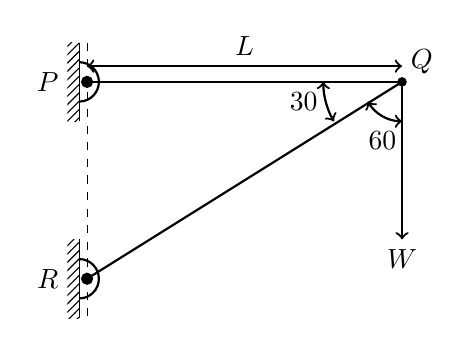
\begin{tikzpicture}
\fill[thick, pattern=north east lines] (-0.25,2.5) rectangle (-0.1,3.5);
\fill[thick, pattern=north east lines] (-0.25,0) rectangle (-0.1,1);
\draw[thick] (-0.1,2.75) arc[start angle=-90, end angle=90, radius=0.25];
\draw[thick] (-0.1,0.25) arc[start angle=-90, end angle=90, radius=0.25];
\draw[dashed] (0,3.5) -- (0,0);
\draw (-0.1,2.5) -- (-0.1,3.5);
\draw (-0.1,0) -- (-0.1,1);
\filldraw (0,3) circle (2pt);
\filldraw (0,0.5) circle (2pt);
\node at (-0.5,3) {$P$};
\node at (-0.5,0.5) {$R$};
\filldraw (4,3) circle (1.5pt);
\node at (4.25,3.25) {$Q$};
\draw[thick] (0,3) -- (4,3);
\draw[thick] (0,0.5) -- (4,3);
\draw[thick, ->] (4,3) -- (4,1) node[below] {$W$};
\draw[thick, <->] (0,3.2) -- (4,3.2) node[midway, above] {$L$};
\draw[thick, <->] (4,2.5) arc[start angle=270, end angle=210, radius=0.5];
\node at (3.75,2.25) {$60\degree$};
\draw[thick, <->] (3,3) arc[start angle=180, end angle=210, radius=1];
\node at (2.75,2.75) {$30\degree$};
\end{tikzpicture}

\begin{multicols}{2}
\begin{enumerate}
\item $2W$ tensile and $\sqrt{3}W$ compressive
\item $\sqrt{3}W$ tensile and $2W$ compressive
\item $\sqrt{3}W$ compressive and $2W$ tensile
\item $2W$ compressive and $\sqrt{3}W$ tensile
\end{enumerate}
\end{multicols}

\item A horizontal bar with a constant cross-section is subjected to loading as shown in the figure. The Young's moduli for the sections $AB$ and $BC$ are $3E$ and $E$, respectively.
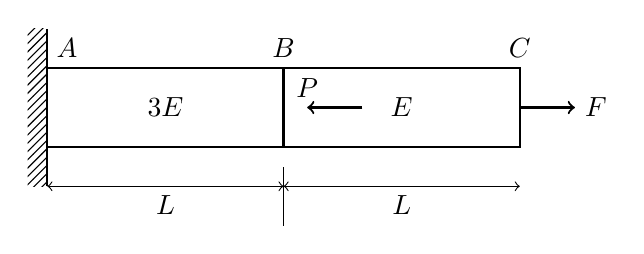
\begin{tikzpicture}
\fill[pattern=north east lines] (-0.25,1.5) rectangle (0,-0.5);
\draw[thick] (0,0) rectangle (3,1) node[midway] {$3E$};
\draw[thick] (3,0) rectangle (6,1) node[midway] {$E$};
\draw[thick] (0,-0.5) -- (0,1.5);
\node at (0.25,1.25) {$A$};
\node at (3,1.25) {$B$};
\node at (6,1.25) {$C$};
\draw[->, thick] (4,0.5) -- (3.3,0.5) node[above] {$P$};
\draw[->, thick] (6,0.5) -- (6.7,0.5) node[right] {$F$};
\draw[<->] (0,-0.5) -- (3,-0.5) node[midway, below] {$L$};
\draw[<->] (3,-0.5) -- (6,-0.5) node[midway, below] {$L$};
\draw (3,-1) -- (3,-0.25);
\end{tikzpicture}

For the deflection at $C$ to be zero, the ratio $P/F$ is \rule{1cm}{0.15mm} \hfill(2016)


\item The figure shows cross-section of a beam subjected to bending. The area moment of inertia (in $mm^{4}$) of this cross-section about its base is \rule{1cm}{0.15mm} \hfill(2016)

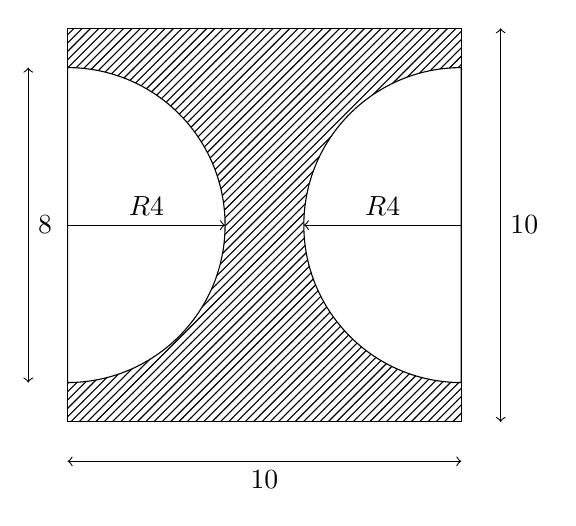
\begin{tikzpicture}
\draw[pattern=north east lines] (0, 0) rectangle (5, 5);
\draw[fill=white] (0, 4.5) arc[start angle=90, end angle=-90, radius=2] -- cycle;
\draw[fill=white] (5, 4.5) arc[start angle=90, end angle=270, radius=2] -- cycle;
\draw[<->] (5.5, 0) -- (5.5, 5) node[midway, right] {10};
\draw[<->] (-0.5, 0.5) -- (-0.5, 4.5) node[midway, right] {8};
\draw[<->] (0, -0.5) -- (5, -0.5) node[midway, below] {10};
\draw[->] (0, 2.5) -- (2,2.5) node[midway, above] {$R4$};
\draw[->] (5, 2.5) -- (3,2.5) node[midway, above] {$R4$};
\end{tikzpicture}

All dimensions are in $mm$


\item A simply-supported beam of length $3L$ is subjected to the loading shown in the figure.

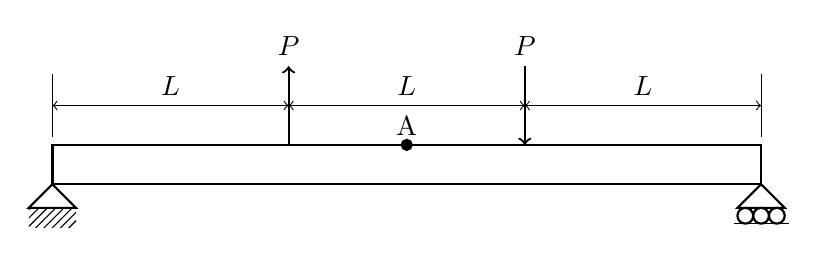
\begin{tikzpicture}
\draw[thick] (0,0) -- (9,0) -- (9,0.5) -- (0,0.5) -- (0,0);
\draw[thick] (0,0) -- (-0.3,-0.3) -- (0.3,-0.3) -- cycle;
\draw[thick] (9,0) -- (8.7,-0.3) -- (9.3,-0.3) -- cycle;
\draw[thick] (8.8,-0.4) circle (0.1); 
\draw[thick] (9,-0.4) circle (0.1);
\draw[thick] (9.2,-0.4) circle (0.1);
\draw[thick,->] (3,0.5) -- (3,1.5) node[above] {$P$};
\draw[thick,->] (6,1.5) -- (6,0.5);
\node at (6,1.75) {$P$};
\draw (0,0.6) -- (0,1.4);
\draw (9,0.6) -- (9,1.4);
\draw[<->] (0,1) -- (3,1) node[midway, above] {$L$};
\draw[<->] (3,1) -- (6,1) node[midway, above] {$L$};
\draw[<->] (6,1) -- (9,1) node[midway, above] {$L$};
\filldraw (4.5,0.5) circle (2pt);
\node at (4.5,0.5) [above] {A};
\fill[pattern=north east lines] (-0.3,-0.55) rectangle (0.3,-0.3);
\draw (8.65,-0.5) -- (9.35,-0.5);
\end{tikzpicture}

It is given that $P=1N$, $L=1m$ and Young's modulus $E=200GPa$. The cross-section is a square with dimension $10mm\times 10mm$. The bending stress (in $Pa$) at the point $A$ located at the top surface of the beam at a distance of $1.5L$ from the left end is \rule{1cm}{0.15mm}\hfill(2016)

(Indicate compressive stress by a negative sign and tensile stress by a positive sign)

\item A slider crank mechanism with crank radius $200mm$ and connecting rod length $800mm$ is shown. The crank is rotating at $600rpm$ in the counterclockwise direction. In the configuration shown, the crank makes an angle of $90\degree$ with the sliding direction of the slider, and a force of $5kN$ is acting on the slider. Neglecting the inertia forces, the turning moment on the crank (in $KN-m$) is \rule{1cm}{0.15mm}\hfill(2016)

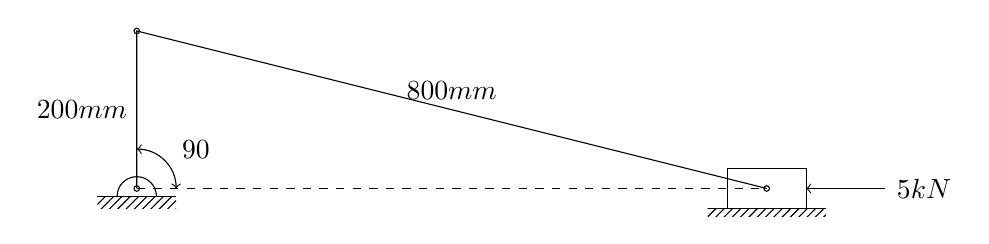
\begin{tikzpicture}
\draw (0,0) -- (0,2) node[midway,left] {$200mm$} -- (8,0) node[midway,above] {$800mm$};
\draw[dashed] (0,0) -- (8,0);
\draw (-0.5,-0.1) -- (0.5,-0.1);
\fill[pattern=north east lines] (-0.5,-0.25) rectangle (0.5,-0.1);
\draw (-0.25,-0.1) arc (180:0:0.25);
\draw (7.25,-0.25) -- (8.75,-0.25);
\fill[pattern=north east lines] (7.25,-0.35) rectangle (8.75,-0.25);
\draw (7.5,-0.25) rectangle (8.5,0.25);
\draw (0,0) circle (1pt);
\draw (8,0) circle (1pt);
\draw[->] (9.5,0) -- (8.5,0);
\node at (10,0) {$5kN$};
\draw[<->] (0.5,0) arc (0:90:0.5);
\node at (0.75,0.5) {$90\degree$};
\draw (0,2) circle (1pt);
\end{tikzpicture}


\item In the gear train shown, gear $3$ is carried on arm $5$. Gear $3$ meshes with gear $2$ and gear $4$. The number of teeth on gear $2$, $3$ and $4$ are $60$, $20$ and $100$ respectively. If gear $2$ is fixed and gear $4$ rotates with an angular velocity of $100rpm$ in the counterclockwise direction, the angular speed of arm $5$ (in $rpm$) is\hfill(2016)

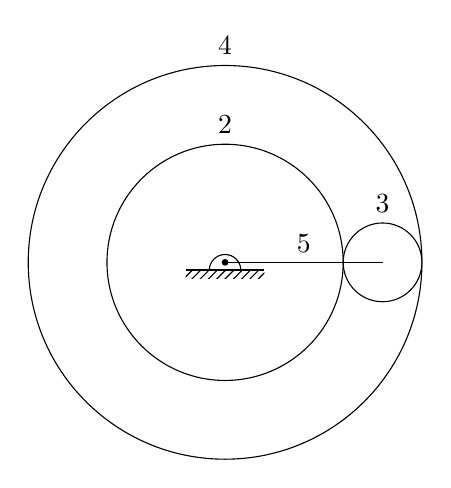
\begin{tikzpicture}
\draw (0,0) circle (2.5cm);
\draw (0,0) circle (1.5cm);
\draw (2,0) circle (0.5cm);
\draw[thick] (-0.5,-0.1) -- (0.5,-0.1);
\fill[pattern=north east lines] (-0.5, -0.2) -- (0.5,-0.2) -- (0.5, -0.1) -- (-0.5,-0.1);
\draw (0,0) -- (2,0) node[midway,above] {$5$};
\draw (-0.2,-0.1) arc[start angle=180, end angle=0, radius=0.2cm];
\filldraw (0,0) circle (1pt);
\node at (0,1.75) {$2$};
\node at (0,2.75) {$4$};
\node at (2,0.75) {$3$};
\end{tikzpicture}
\begin{multicols}{2}
\begin{enumerate}
\item $166.7$ counterclockwise
\item $166.7$ clockwise
\item $62.5$ counterclockwise
\item $62.5$ clockwise
\end{enumerate}
\end{multicols}


\item A solid disc with radius $a$ is connected to a spring at a point $d$ above the center of the disc. The other end of the spring is fixed to the vertical wall. The disc is free to roll without slipping on the ground. The mass of the disc is $M$ and the spring constant is $K$. The polar moment of inertia for the disc about its centre is $J=\frac{Ma^{2}}{2}$.
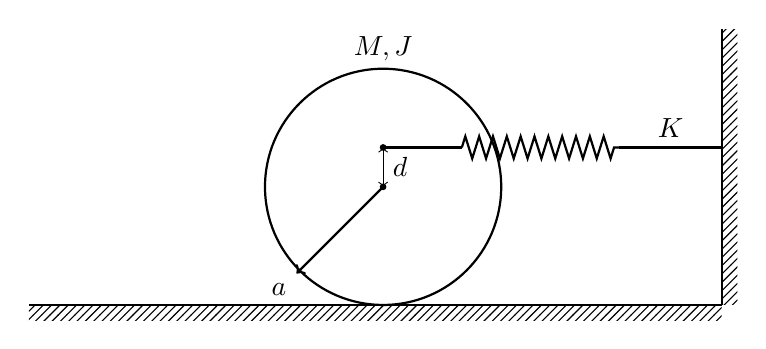
\begin{tikzpicture}
\fill[pattern=north east lines] (-4.5, -1.7) rectangle (4.3, -1.5);
\fill[pattern=north east lines] (4.3, -1.5) rectangle (4.5, 2);
\draw[thick] (-4.5, -1.5) -- (4.3, -1.5);
\draw[thick] (4.3, -1.5) -- (4.3, 2);
\draw[thick] (0,0) circle (1.5cm);
\filldraw (0,0) circle (1pt);
\filldraw (0,0.5) circle (1pt);
\draw[->, thick] (0,0) -- (-1.1,-1.1) node[below left] {$a$};
\draw[thick] (0, 0.5) -- (1, 0.5);
\draw[thick, decorate, decoration={zigzag, segment length=5, amplitude=4}] (1, 0.5) -- (3, 0.5);
\draw[thick] (3, 0.5) -- (4.3, 0.5) node[midway, above] {$K$};
\node at (0,1.75) {$M,J$};
\draw[<->] (0,0) -- (0,0.5) node[midway, right] {$d$};
\end{tikzpicture}

The natural frequency of this system in $rad/s$ is given by\hfill(2016)
\begin{multicols}{2}
\begin{enumerate}
\item $\sqrt{\frac{2K\brak{a+d}^{2}}{3Ma^{2}}}$
\item $\sqrt{\frac{2K}{3M}}$
\item $\sqrt{\frac{2K\brak{a+d}^{2}}{Ma^{2}}}$
\item $\sqrt{\frac{K\brak{a+d}^{2}}{Ma^{2}}}$
\end{enumerate}
\end{multicols}


\item The principal stresses at a point inside a solid object are $\sigma_{1}=100MPa$, $\sigma_{2}=100 MPa$ and $\sigma_{3}=0MPa$. The yield strength of the material is $200MPa$. The factor of safety calculated using Tresca (maximum shear stress) theory is $n_{T}$ and the factor of safety calculated using von Mises (maximum distortional energy) theory is $n_{V}$. Which one of the following relations is TRUE?\hfill(2016)
\begin{multicols}{2}
\begin{enumerate}
\item $n_{T}=\brak{\frac{\sqrt{3}}{2}}n_{V}$
\item $n_{T}=\brak{\sqrt{3}}n_{V}$
\item $n_{T}=n_{V}$
\item $n_{V}=\brak{\sqrt{3}}n_{T}$
\end{enumerate}
\end{multicols}


\item An inverted U-tube manometer is used to measure the pressure difference between two pipes $A$ and $B$, as shown in the figure. Pipe $A$ is carrying oil (specific gravity$=0.8$) and pipe $B$ is carrying water. The densities of air and water are and $1.16kg/m^{3}$ and $1000kg/m^{3}$, respectively. The pressure difference between pipes $A$ and $B$ is \rule{1cm}{0.15mm} $kPa$.

Acceleration due to gravity $g=10m/s^{2}$.\hfill(2016)

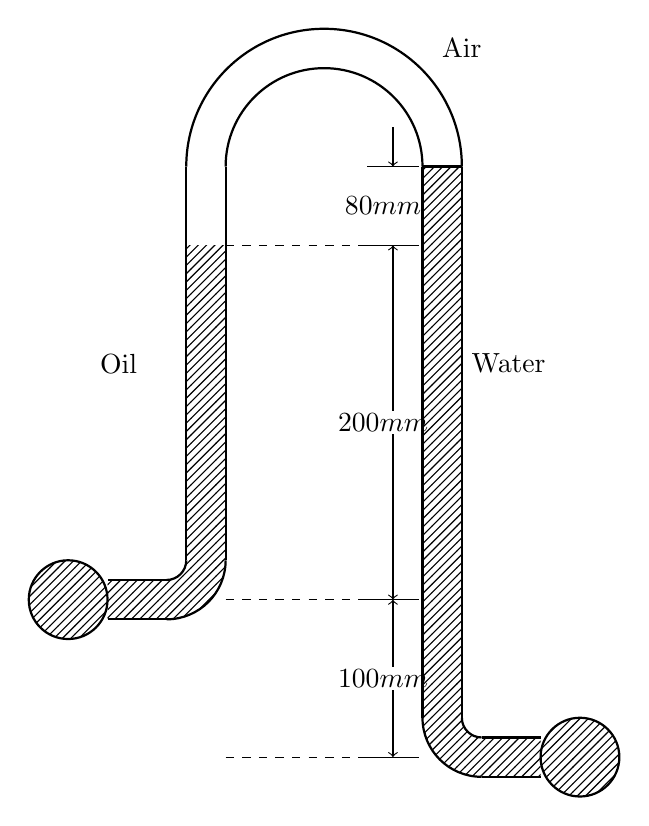
\begin{tikzpicture}
\draw[thick] (0.5,0) -- (0.5,5);
\draw[thick] (1,0) -- (1,5);
\draw[thick] (3.5,-2) -- (3.5,5);
\draw[thick] (4,-2) -- (4,5);
\draw[thick] (1,5) arc[start angle=180, end angle=0, radius=1.25cm];
\draw[thick] (0.5,5) arc[start angle=180, end angle=0, radius=1.75cm];
\node at (4,6.5) {Air};
\node[left] at (0,2.5) {Oil};
\node[right] at (4,2.5) {Water};
\draw[dashed] (1,4) -- (3.5,4);
\draw[dashed] (1,-0.5) -- (3.5,-0.5);
\draw[dashed] (1,-2.5) -- (3.5,-2.5);
\fill[pattern=north east lines] (0.5,0) rectangle (1,4);
\fill[pattern=north east lines] (4,-2) rectangle (3.5,5);
\draw[thick] (-1,-0.5) circle (0.5cm);
\fill[pattern=north east lines] (-1,-0.5) circle (0.5cm);
\draw[thick] (0.5,0) arc[start angle=0, end angle=-90, radius=0.25cm];
\draw[thick] (0.25,-0.75) arc (-90:0:0.75);
\fill[thick,pattern=north east lines] (0.5,0) arc[start angle=0, end angle=-90, radius=0.25cm] -- (0.25,-0.75) arc (-90:0:0.75);
\draw[thick] (5.5,-2.5) circle (0.5cm);
\fill[pattern=north east lines] (5.5,-2.5) circle (0.5cm);
\draw[thick] (3.5,-2) arc[start angle=180, end angle=270, radius=0.75cm];
\draw[thick] (4.25,-2.25) arc[start angle=270, end angle=180, radius=0.25cm];
\fill[thick,pattern=north east lines] (3.5,-2) arc[start angle=180, end angle=270, radius=0.75cm] -- (4.25,-2.25) arc[start angle=270, end angle=180, radius=0.25cm];
\draw[thick] (0.25,-0.75) -- (-0.5,-0.75);
\draw[thick] (0.25,-0.25) -- (-0.5,-0.25);
\fill[pattern=north east lines] (0.25,-0.75) rectangle (-0.5,-0.25);
\draw[thick] (4.25,-2.75) -- (5,-2.75);
\draw[thick] (4.25,-2.25) -- (5,-2.25);
\fill[pattern=north east lines] (4.25,-2.75) rectangle (5,-2.25);
\draw[thick] (3.5,5) -- (4,5);
\draw[->] (3.125,5.5) -- (3.125,5);
\draw (3.45,5) -- (2.8,5);
\draw (3.45,4) -- (2.8,4);
\draw (3.45,-0.5) -- (2.8,-0.5);
\draw (3.45,-2.5) -- (2.8,-2.5);
\node at (3,4.5) {$80mm$};
\node at (3,1.75) {$200mm$};
\node at (3,-1.5) {$100mm$};
\draw[->] (3.125,1.9) -- (3.125,4);
\draw[->] (3.125,1.6) -- (3.125,-0.5);
\draw[->] (3.125,-1.35) -- (3.125,-0.5);
\draw[->] (3.125,-1.65) -- (3.125,-2.5);
\end{tikzpicture}



\item Oil (kinematic viscosity, $v_{oil}=1.0\times 10^{-5}m^{2}/s$) flows through a pipe of $0.5m$ diameter with a velocity of $10m/s$. Water (kinematic viscosity, $v_{w}=0.89\times 10^{-6}m^{2}/s$) is flowing through a model pipe of diameter $20mm$. For satisfying the dynamic similarity, the velocity of water (in $m/s$) is \rule{1cm}{0.15mm}\hfill(2016)


\item A steady laminar boundary layer is formed over a flat plate as shown in the figure. The free stream velocity of the fluid is $U_{o}$. The velocity profile at the inlet $a-b$ is uniform, while that at a downstream location $c-d$ is given by $u=U_{o}\sbrak{2\brak{\frac{y}{\delta}}-\brak{\frac{y}{\delta}}^{2}}$.

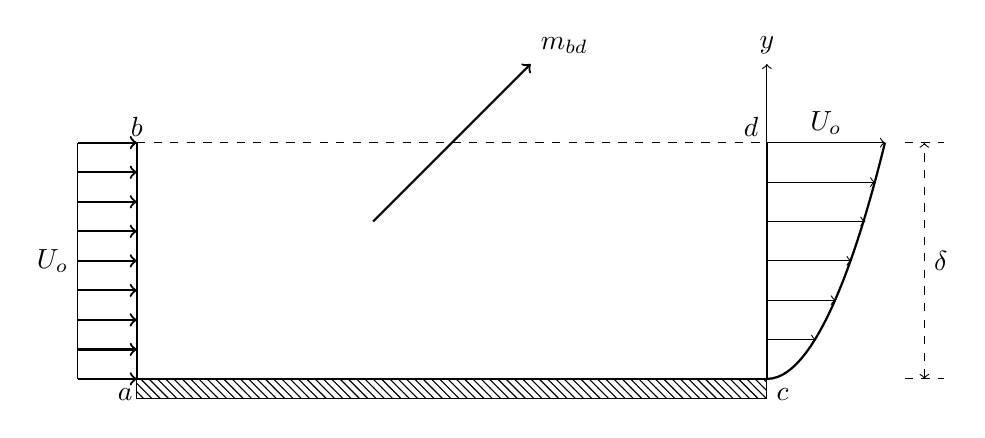
\begin{tikzpicture}
\draw (-0.75,0) -- (-0.75,3);
\foreach \y in {0,0.375,0.75,...,2.625,3} {
\draw[->,thick] (-0.75,\y) -- (0,\y);
}
\draw[thick] (0,3) -- (0,0) -- (8,0) -- (8,3);
\draw[pattern=north west lines] (0,0) rectangle (8,-0.25);
\node[left] at (-0.75,1.5) {$U_o$};
\node at (8.75,3.25) {$U_o$};
\node at (-0.15,-0.2) {$a$};
\node at (0,3.2) {$b$};
\node at (8.2,-0.2) {$c$};
\node at (7.8,3.2) {$d$};
\draw[->] (8,3) -- (8,4) node[above] {$y$};
\draw[->,thick] (3,2) -- (5,4) node[above right] {$m_{bd}$};
\draw[dashed] (0,3) -- (8,3);
\draw[thick] (8,0) parabola (9.5,3);
\draw[dashed] (9.75,0) -- (10.25,0);
\draw[dashed] (9.75,3) -- (10.25,3);
\draw[<->,dashed] (10,0) -- (10,3) node[midway, right] {$\delta$};
\draw[->] (8,3) -- (9.5,3);
\draw[->] (8,2.5) -- (9.375
,2.5);
\draw[->] (8,2) -- (9.25,2);
\draw[->] (8,1.5) -- (9.075,1.5);
\draw[->] (8,1) -- (8.875,1);
\draw[->] (8,0.5) -- (8.625,0.5);
\end{tikzpicture}

The ratio of the mass flow rate, $m_{bd}$, leaving through the horizontal section $b-d$ to that entering through the vertical section $a-b$ is \rule{1cm}{0.15mm}\hfill(2016)


\item A steel ball of $10mm$ diameter at $1000K$ is required to be cooled to $350K$ by immersing it in a water environment at $300K$. The convective heat transfer coefficient is $1000 W/m^{2}-K$. Thermal conductivity of steel is $40W/m-K$. The time constant for the cooling process $\tau$ is $16s$. The time required (in $s$) to reach the final temperature is \rule{1cm}{0.15mm}\hfill(2016)